% uid: ""
% school: "college"
% level: "7eme"
% chapter: "التناظر المحوري"
% chapter_slug: "symetrie-axiale"
% title: "محاور التناظر"
% difficulty: "Facile"
% tags: ["axes-de-symetrie", "figures-usuelles", "quadrillage"]
% provenance: "own"
% batch: "2026-11-27-symetrie-axiale-7eme"
% Exercice 4/10 de la série 7ème « التناظر المحوري » (statement + \axsol + solution). Compiler avec XeLaTeX + axiomath.sty (+ axiomaths-logo.png).
\documentclass[12pt,a4paper]{article}
\usepackage[level=7b,color=0F766E]{axiomath}
\newcommand{\cm}{\,\mathrm{cm}}
\axsetup{title={التناظر المحوري}, corrige}

\begin{document}

\begin{corr}[title={محاور التناظر}, stars=1, source={Axiomaths}]
\begin{enumerate}
  \item أتمم الجدول :
  \begin{center}
  \renewcommand{\arraystretch}{1.5}
  \begin{tabular}{|c|c|}
    \hline
    الشكل & عدد محاور التناظر \\ \hline
    قطعة مستقيم & \phantom{لا نهاية لا نهاية} \\ \hline
    زاوية & \\ \hline
    مستطيل (غير مربع) & \\ \hline
    مربع & \\ \hline
    مثلث متقايس الضلعين (غير متقايس الأضلاع) & \\ \hline
    دائرة & \\ \hline
  \end{tabular}
  \end{center}
  \item ارسم محاور تناظر كل شكل من الأشكال التالية إن وُجدت.
  \begin{center}
  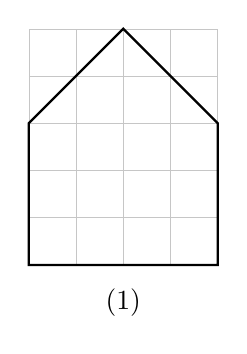
\begin{tikzpicture}[scale=0.6]
    \draw[gray!45,very thin] (0,0) grid (4,5);
    \draw[thick] (0,0)--(4,0)--(4,3)--(2,5)--(0,3)--cycle;
    \node at (2,-0.8) {(1)};
  \end{tikzpicture}
  \qquad
  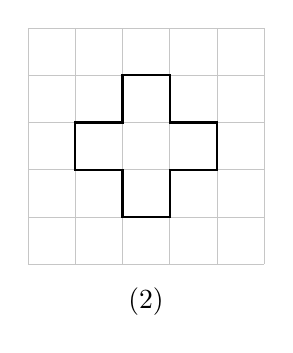
\begin{tikzpicture}[scale=0.6]
    \draw[gray!45,very thin] (-1,-1) grid (4,4);
    \draw[thick] (1,0)--(2,0)--(2,1)--(3,1)--(3,2)--(2,2)--(2,3)--(1,3)--(1,2)--(0,2)--(0,1)--(1,1)--cycle;
    \node at (1.5,-1.8) {(2)};
  \end{tikzpicture}
  \qquad
  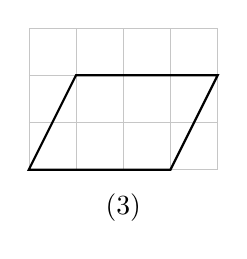
\begin{tikzpicture}[scale=0.6]
    \draw[gray!45,very thin] (0,0) grid (4,3);
    \draw[thick] (0,0)--(3,0)--(4,2)--(1,2)--cycle;
    \node at (2,-0.8) {(3)};
  \end{tikzpicture}
  \end{center}
\end{enumerate}
\axsol
\begin{enumerate}[itemsep=14pt]
  \item\leavevmode
  \begin{prop}[محور تناظر شكل]
  المستقيم $\Delta$ محور تناظر لشكل معناه : \ib{مناظر الشكل بالنسبة إلى $\Delta$ هو الشكل نفسه} (إذا طوينا الورقة على $\Delta$ ينطبق نصفا الشكل).
  \end{prop}
  \begin{center}
  \renewcommand{\arraystretch}{1.5}
  \begin{tabular}{|c|c|}
    \hline
    الشكل & عدد محاور التناظر \\ \hline
    قطعة مستقيم & $2$ : محورها والمستقيم الحامل لها \\ \hline
    زاوية & $1$ : المستقيم الحامل لمنصّفها \\ \hline
    مستطيل (غير مربع) & $2$ \\ \hline
    مربع & $4$ \\ \hline
    مثلث متقايس الضلعين (غير متقايس الأضلاع) & $1$ \\ \hline
    دائرة & لا نهاية (كل مستقيم يمرّ من المركز) \\ \hline
  \end{tabular}
  \end{center}
  \item
  \begin{itemize}[itemsep=8pt]
    \item الشكل (1) : \ib{محور واحد}، المستقيم الرأسي المارّ من القمة.
    \item الشكل (2) : \ib{4 محاور}، المستقيم الرأسي والمستقيم الأفقي المارّان من المركز، والقطران.
    \item الشكل (3) : \ib{لا محور له}. إذا طويناه على أي مستقيم لا ينطبق نصفاه.
  \end{itemize}
  \begin{center}
  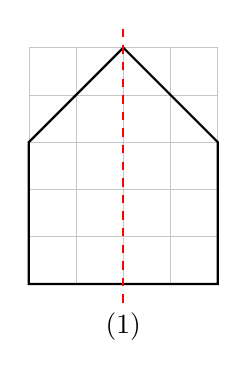
\begin{tikzpicture}[scale=0.6]
    \draw[gray!45,very thin] (0,0) grid (4,5);
    \draw[thick] (0,0)--(4,0)--(4,3)--(2,5)--(0,3)--cycle;
    \draw[red,thick,dashed] (2,-0.4)--(2,5.4);
    \node at (2,-0.9) {(1)};
  \end{tikzpicture}
  \qquad
  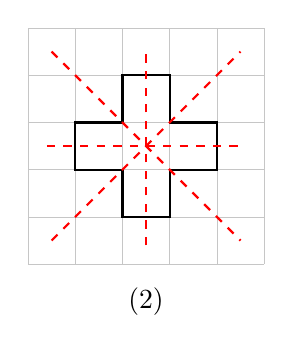
\begin{tikzpicture}[scale=0.6]
    \draw[gray!45,very thin] (-1,-1) grid (4,4);
    \draw[thick] (1,0)--(2,0)--(2,1)--(3,1)--(3,2)--(2,2)--(2,3)--(1,3)--(1,2)--(0,2)--(0,1)--(1,1)--cycle;
    \draw[red,thick,dashed] (1.5,-0.6)--(1.5,3.6);
    \draw[red,thick,dashed] (-0.6,1.5)--(3.6,1.5);
    \draw[red,thick,dashed] (-0.5,-0.5)--(3.5,3.5);
    \draw[red,thick,dashed] (-0.5,3.5)--(3.5,-0.5);
    \node at (1.5,-1.8) {(2)};
  \end{tikzpicture}
  \qquad
  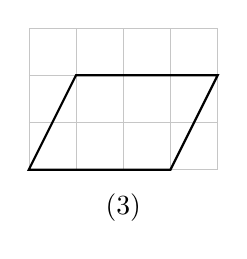
\begin{tikzpicture}[scale=0.6]
    \draw[gray!45,very thin] (0,0) grid (4,3);
    \draw[thick] (0,0)--(3,0)--(4,2)--(1,2)--cycle;
    \node at (2,-0.8) {(3)};
  \end{tikzpicture}
  \end{center}
  \textbf{انتبه :} الشكل (3) متوازي أضلاع عادي. القطر ليس محور تناظر له : نتحقق بالطي.
\end{enumerate}
\end{corr}

\end{document}
